\documentclass[12pt,xcolor=dvipsnames]{beamer}

%%%%%% Packages %%%%%%%%%%%%%%%%%%%%%%%%%%%%%%%%%%%%%%%%%%%%%%%%%%%%%
%\usepackage[overlay, absolute]{textpos}
\usepackage[utf8]{inputenc}
\usepackage[T1]{fontenc}
\usepackage{amssymb,amsmath}
\usepackage{mathtools}
\usepackage{tikz}
%\usepackage{upgreek}
%\usepackage{scalerel}

\usetikzlibrary{matrix,fit,positioning}

%\usetikzlibrary{arrows,,tikzmark,shapes.callouts, shapes.multipart}
%%%%%%%%%%%%%%%%%%%%%%%%%%%%%%%%%%%%%%%%%%%%%%%%%%%%%%%%%%%%%%%%%%%%

%%%%%% Macros %%%%%%%%%%%%%%%%%%%%%%%%%%%%%%%%%%%%%%%%%%%%%%%%%%%%%%%
\newcommand{\Matrix}[5]{\big[#1 \leftarrow #2\,\times\,#3 \leftarrow #4\big]\,#5}
\newcommand{\MatrixSimp}[3]{\big[#1 \,\times\,#2 \big]\,#3}
\newcommand{\splash}[2][]{\begin{frame}\begin{center}\resizebox{0.9\textwidth}{!}{#2}\end{center}\begin{tikzpicture}[remember picture,overlay]\node at (current page.south west) [above right] {{\tiny \textcolor{gray}{#1}}}; \end{tikzpicture}\end{frame}}
\newcommand{\splashTitle}[1]{{\setbeamercolor{background canvas}{bg=black}\begin{frame}\begin{center}\resizebox{0.8\textwidth}{!}{\textcolor{white}{#1}}\end{center}\end{frame}}\addtocounter{framenumber}{-1}}
%%%%%%%%%%%%%%%%%%%%%%%%%%%%%%%%%%%%%%%%%%%%%%%%%%%%%%%%%%%%%%%%%%%%%

%%%%%% Tweaking %%%%%%%%%%%%%%%%%%%%%%%%%%%%%%%%%%%%%%%%%%%%%%%%%%%%%
\beamertemplatenavigationsymbolsempty

\usecolortheme{lily}
\setbeamercovered{invisible}
\defbeamertemplate*{footline}{my theme}
{
  \leavevmode%
  \hbox{%
    \usebeamerfont{date in head/foot}
    \hspace*{0.97\paperwidth}\raisebox{2pt}{\insertframenumber{}}}
  \vskip0pt%
}
%%%%%%%%%%%%%%%%%%%%%%%%%%%%%%%%%%%%%%%%%%%%%%%%%%%%%%%%%%%%%%%%%%%%%


\begin{document}

% \frame{\titlepage} %% done manually
%
{
%\usebackgroundtemplate{%
%\tikz\node[opacity=0.40, inner sep=0] {\includegraphics[height=\paperheight]{pics/taipei_tree}};}
\begin{frame}[plain,t]
\vspace*{.9cm}
\begin{center}
\textbf{{\Large LabMate: a prospectus for types for MATLAB}}
\\[0.2cm]
\vspace*{0.9cm}

{\large  \textbf{Georgi Nakov, Conor Mc Bride, and Fredrik Nordvall Forsberg}}\\
{\normalsize \textbf{University of Strathclyde, Glasgow, Scotland}}

\vspace*{0.4cm}

\vspace*{0.8cm}

\normalsize

\textbf{NPL Data Science Seminar, Teddington}

\medskip

\textbf{12 September 2024}

\end{center}
\end{frame}
}

\setcounter{framenumber}{0}

\section{I}
\splashTitle{(I)}
\splash{Conor}
\splash{Fred}
\splash{Georgi}
\splash{MSP}
\splash{dependent}
\splash{conquest}
\splash{infection}

\section{II}
\splashTitle{(II)}
\splash{articulacy}
\splash{listening}
\splash{talking}
\splash{sense}
\splash{model}
\splash{deep}
\splash{mathematics}

\section{III}
\splashTitle{(III)}
\splash{MATLAB}
\splash{comments}
\splash{LabMate}
\splash[demo\_3\_0\_hello\_labmate.m]{transducer}
\splash{collaborator}
\splash{stick}
\splash{carrot}

\section{IV}
\splashTitle{(IV)}
\splash{dark}
\splash{dance}
\splash{rules}
\splash[Matlab]{space}
\splash[demo\_4\_0\_renaming\_simple.m, demo\_4\_1\_nested\_captured.m]{scope}

\section{V}
\splashTitle{(V)}
\splash{expect}
\splash{gradualism}
\splash[demo\_5\_0\_zen\_error.m]{zen}
\splash{locality}
\splash[demo\_5\_1\_cubit.m]{dimension}
\splash{units}

\splash{mass $\cdot$ length/time}
\splash{group}

\splash{$Q(\mathsf{M}\cdot\mathsf{L}/\mathsf{T})$}
\splash{${}+{} : Q(d) \to Q(d) \to Q(d)$}
\splash{${}\ast{} : Q(d) \to Q(e) \to Q(d \cdot e)$}

\splash{[Kennedy 1995]}
\splash{F\#}
\splash{Pint}

\begin{frame}
  \begin{center}
    \includegraphics[scale=0.7]{hart}
  \end{center}
\end{frame}

\splash{
$\begin{pmatrix}
  d & d & d \\
  d & d & d \\
  d & d & d \\
  d & d & d
\end{pmatrix}
\; ?
$}

\splash{
  $\begin{pmatrix}
    d & e & f \\
    g & h & i \\
    j & k & l \\
    m & n & o
  \end{pmatrix}
\; ?$}

\splash{
  $\begin{pmatrix}
    d_{1,1} & d_{1,2} & d_{1,3} \\
    d_{2,1} & d_{2,2} & d_{2,3} \\
    d_{3,1} & d_{3,2} & d_{3,3} \\
    d_{4,1} & d_{4,2} & d_{4,3}
  \end{pmatrix}$}

\begin{frame}

  {\Large
  \[
    \Matrix{i}{[r_1, \ldots, r_n]}{j}{[c_1, \ldots, c_m]}{C(i, j)}
  \]
}
\bigskip

\begin{center}
  \resizebox{0.8\textwidth}{!}{
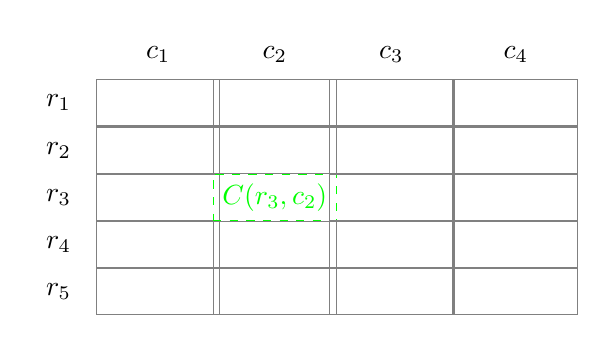
\begin{tikzpicture}[ampersand replacement=\&]
  \matrix[entry/.style={draw, gray}]
  {
    \&[2mm] \node{$c_1$}; \&[-1mm] \node {$c_2$}; \&[-1mm] \node {$c_3$}; \& \node {$c_4$}; \\[1mm]
    \node {$r_1$}; \& \node[entry]{\phantom{$C(r_3, c_2)$}}; \& \node[entry]{\phantom{$C(r_3, c_2)$}}; \& \node[entry]{\phantom{$C(r_3, c_2)$}}; \& \node[entry]{\phantom{$C(r_3, c_2)$}}; \\
    \node {$r_2$}; \& \node[entry]{\phantom{$C(r_3, c_2)$}}; \& \node[entry]{\phantom{$C(r_3, c_2)$}}; \& \node[entry]{\phantom{$C(r_3, c_2)$}}; \& \node[entry]{\phantom{$C(r_3, c_2)$}}; \\
    \node {$r_3$}; \& \node[entry]{\phantom{$C(r_3, c_2)$}}; \& \node[draw,dashed,green]{$C(r_3, c_2)$}; \& \node[entry]{\phantom{$C(r_3, c_2)$}}; \& \node[entry]{\phantom{$C(r_3, c_2)$}}; \\
    \node {$r_4$}; \& \node[entry]{\phantom{$C(r_3, c_2)$}}; \& \node[entry]{\phantom{$C(r_3, c_2)$}}; \& \node[entry]{\phantom{$C(r_3, c_2)$}}; \& \node[entry]{\phantom{$C(r_3, c_2)$}}; \\
    \node {$r_5$}; \& \node[entry]{\phantom{$C(r_3, c_2)$}}; \& \node[entry]{\phantom{$C(r_3, c_2)$}}; \& \node[entry]{\phantom{$C(r_3, c_2)$}}; \& \node[entry]{\phantom{$C(r_3, c_2)$}}; \\
  };
\end{tikzpicture}
}
\end{center}
\end{frame}

\begin{frame}

\resizebox{0.8\textwidth}{!}{$\Matrix{i}{[[], [], [], []]}{j}{[[], []]}{\textsf{double}}$}

\bigskip

\uncover<2->{
  \begin{center}
    {\Huge =}
  \end{center}

  \bigskip

  \resizebox{0.8\textwidth}{!}{$\MatrixSimp{4}{2}{\textsf{double}}$}
}
\end{frame}

\splash{$\Matrix{r}{[d_1, \ldots, d_n]}{c}{[e_1, \ldots, e_m]}{Q(r/c)}$}

\begin{frame}

\scalebox{0.7}{%
    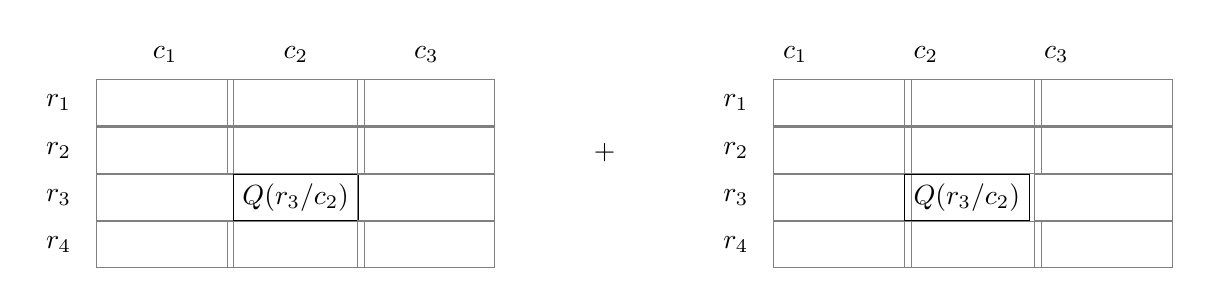
\begin{tikzpicture}[ampersand replacement=\&]
  \matrix[entry/.style={draw, gray}] (l)
  {
    \&[2mm] \node{$c_1$}; \&[-1mm] \node {$c_2$}; \&[-1mm] \node {$c_3$}; \\[1mm]
    \node {$r_1$}; \& \node[entry]{\phantom{$Q(r_3/m_2)$}}; \& \node[entry]{\phantom{$Q(r_3/m_2)$}}; \& \node[entry]{\phantom{$Q(r_3/m_2)$}}; \\
    \node {$r_2$}; \& \node[entry]{\phantom{$Q(r_3/m_2)$}}; \& \node[entry]{\phantom{$Q(r_3/m_2)$}}; \& \node[entry]{\phantom{$Q(r_3/m_2)$}}; \\
    \node {$r_3$}; \& \node[entry]{\phantom{$Q(r_3/m_2)$}}; \& \node[draw]{$Q(r_3/c_2)$}; \& \node[entry]{\phantom{$Q(r_3/m_2)$}}; \\
    \node {$r_4$}; \& \node[entry]{\phantom{$Q(r_3/m_2)$}}; \& \node[entry]{\phantom{$Q(r_3/m_2)$}}; \& \node[entry]{\phantom{$Q(r_3/m_2)$}}; \\
  };
\node[right = of l] (p) {+} ;
\matrix[right = of p,entry/.style={draw, gray}]
  {
    \&[2mm] \node{$c_1$}; \&[-1mm] \node {$c_2$}; \&[-1mm] \node {$c_3$}; \\[1mm]
    \node {$r_1$}; \& \node[entry]{\phantom{$Q(r_3/m_2)$}}; \& \node[entry]{\phantom{$Q(r_3/m_2)$}}; \& \node[entry]{\phantom{$Q(r_3/m_2)$}}; \\
    \node {$r_2$}; \& \node[entry]{\phantom{$Q(r_3/m_2)$}}; \& \node[entry]{\phantom{$Q(r_3/m_2)$}}; \& \node[entry]{\phantom{$Q(r_3/m_2)$}}; \\
    \node {$r_3$}; \& \node[entry]{\phantom{$Q(r_3/m_2)$}}; \& \node[draw]{$Q(r_3/c_2)$}; \& \node[entry]{\phantom{$Q(r_3/m_2)$}}; \\
    \node {$r_4$}; \& \node[entry]{\phantom{$Q(r_3/m_2)$}}; \& \node[entry]{\phantom{$Q(r_3/m_2)$}}; \& \node[entry]{\phantom{$Q(r_3/m_2)$}}; \\
  };
\end{tikzpicture}
}
\end{frame}

\begin{frame}
\scalebox{0.7}{%
    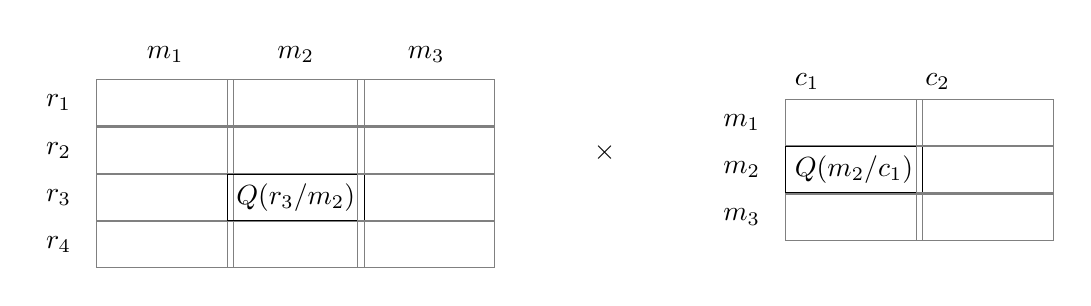
\begin{tikzpicture}[ampersand replacement=\&]
  \matrix[entry/.style={draw, gray}] (l)
  {
    \&[2mm] \node{$m_1$}; \&[-1mm] \node {$m_2$}; \&[-1mm] \node {$m_3$}; \\[1mm]
    \node {$r_1$}; \& \node[entry]{\phantom{$Q(r_3/m_2)$}}; \& \node[entry]{\phantom{$Q(r_3/m_2)$}}; \& \node[entry]{\phantom{$Q(r_3/m_2)$}}; \\
    \node {$r_2$}; \& \node[entry]{\phantom{$Q(r_3/m_2)$}}; \& \node[entry]{\phantom{$Q(r_3/m_2)$}}; \& \node[entry]{\phantom{$Q(r_3/m_2)$}}; \\
    \node {$r_3$}; \& \node[entry]{\phantom{$Q(r_3/m_2)$}}; \& \node[draw]{$Q(r_3/m_2)$}; \& \node[entry]{\phantom{$Q(r_3/m_2)$}}; \\
    \node {$r_4$}; \& \node[entry]{\phantom{$Q(r_3/m_2)$}}; \& \node[entry]{\phantom{$Q(r_3/m_2)$}}; \& \node[entry]{\phantom{$Q(r_3/m_2)$}}; \\
  };
\node[right = of l] (p) {$\times$} ;
\matrix[right = of p,entry/.style={draw, gray}]
  {
    \&[2mm] \node{$c_1$}; \&[-1mm] \node {$c_2$}; \\
    \node {$m_1$}; \& \node[entry]{\phantom{$Q(r_3/m_2)$}}; \& \node[entry]{\phantom{$Q(r_3/m_2)$}}; \\
    \node {$m_2$}; \& \node[draw]{$Q(m_2/ c_1)$}; \& \node[entry]{\phantom{$Q(r_3/m_2)$}}; \\
    \node {$m_3$}; \& \node[entry]{\phantom{$Q(r_3/m_2)$}}; \& \node[entry]{\phantom{$Q(r_3/m_2)$}}; \\
  };
\end{tikzpicture}
}
\begin{tikzpicture}[remember picture,overlay]\node at (current page.south west) [above right] {\scalebox{0.7}{\tiny \textcolor{gray}{demo\_5\_2\_dim\_add.m, demo\_5\_3\_dim\_mult.m, demo\_5\_4\_hello\_labmate.m, demo\_5\_5\_hello\_dimensions.m}}}; \end{tikzpicture}
\end{frame}


%----------------------------------

\section{VI}
\splashTitle{(VI)}
\splash{hat}
\splash{tree}
\splash{concurrent}
\splash{opportunist}
\splash{postponement}
\splash{resumption}
\splash{news}

\section{VII}
\splashTitle{(VII)}
\splash{algebra}
\splash{pasting}
\splash{flow}
\splash{revolution}
\splash{corners}
\splash{normalise}

\section{VIII}
\splashTitle{(VIII)}
\splash{backlog}
\splash{beans}
\splash{breadth}
\splash{business}
\splash{blackmail}
\splash{bait}

\section{IX}
\splashTitle{(IX)}
\splash{time}
\splash{tools}
\splash{urine}
\splash{trials}
\splash{training}
\splash{thanks}

\end{document}



\end{document}
